\documentclass[tikz, convert={outext=.svg,pdf2svg}]{standalone}

\usepackage{tikz,amsmath, amssymb,bm,color}
\usetikzlibrary{shapes,arrows}
\usetikzlibrary{calc}

\definecolor{myblue}{RGB}{175, 204, 233}

\begin{document}
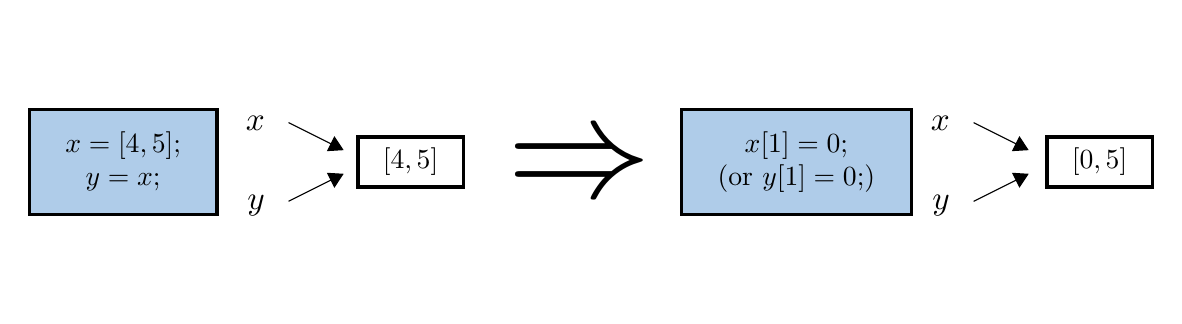
\begin{tikzpicture}

\tikzstyle{square} = [draw,outer sep=7,inner sep=3,minimum size=10,line width=1, 
very thick, draw=black!100, top color=white,bottom color=white]
\tikzstyle{white-b} = [draw,outer sep=7,inner sep=7,minimum size=20,line width=1, 
very thick, draw=blue!25, top color=blue!25, bottom color=blue!25]
\tikzstyle{gray-b} = [draw,outer sep=7,inner sep=7,minimum size=20,line width=1, 
very thick, draw=black!100, top color=myblue, bottom color=myblue]
\tikzstyle{black_block} = [draw, text=white, font=\bf
, outer sep=7,inner sep=5,minimum size=20,line width=1,
very thick, draw=black!5, top color=black!50,bottom color=black]
\tikzstyle{gray_block}= [draw,outer sep=7,inner sep=3,minimum size=20,line width=1,very thick, draw=black!95, top color=white,bottom color=blue!25];
\tikzstyle{red_block}= [draw,outer sep=7,inner sep=3,minimum size=20,line width=1,very thick, draw=red!95, top color=white,bottom color=red!25];



\node [gray-b] at (16.4,15.5)  {\begin{tabular}{c} $x=[4,5]$;\\ $y=x;$\end{tabular}};
 

  \draw[-triangle 60]  (18.5,16) -- (19.2,15.65);
\node[anchor=east,scale=1.2] at (18.6,16) {\begin{tabular}{l} $x$ \end{tabular}}; 

 \draw[-triangle 60]  (18.5,15) -- (19.2,15.35);
\node[anchor=east,scale=1.2] at (18.6,15) {\begin{tabular}{l} $y$ \end{tabular}}; 

\node [square, anchor=center] at (20.05,15.5) {\begin{tabular}{c} $[4,5]$\end{tabular}};


\node[anchor=center,scale=5.2] at (22.2,15.5) {\begin{tabular}{l} $\Rightarrow$ \end{tabular}}; 



\node [gray-b] at (24.95,15.5) {\begin{tabular}{c} $x[1]=0$;\\ (or $y[1]=0;$)\end{tabular}};
 

  \draw[-triangle 60]  (27.2,16) -- (27.9,15.65);
\node[anchor=east,scale=1.2] at (27.3,16) {\begin{tabular}{l} $x$ \end{tabular}}; 

 \draw[-triangle 60]  (27.2,15) -- (27.9,15.35);
\node[anchor=east,scale=1.2] at (27.3,15) {\begin{tabular}{l} $y$ \end{tabular}}; 

\node [square, anchor=center] at (28.8,15.5) {\begin{tabular}{c} $[0,5]$\end{tabular}};


\end{tikzpicture}

\end{document}